\section{Durchführung}

\subsection{Bau des Roboterarmes}
\schritt{1}{Den Roboterarm vorbereiten}{
Die Pappe schneidet ihr in acht 30cm lange und 2cm breite Streifen.
Zwei davon werden auf 15cm gekürzt, zwei weitere auf 12cm.\\

Aus den Resten der gekürzten Streifen schneidet ihr zirka 12 kleine Pappquadrate.
Außerdem benötigt ihr vier Pappteile, die ihr wie auf dem Bild zuschneidet, und zwei Pappkreise, deren Durchmesser ungefähr mit der Größe der Reifen übereinstimmt.\\

\begin{figure}[h]
\centering
\parbox{5cm}{
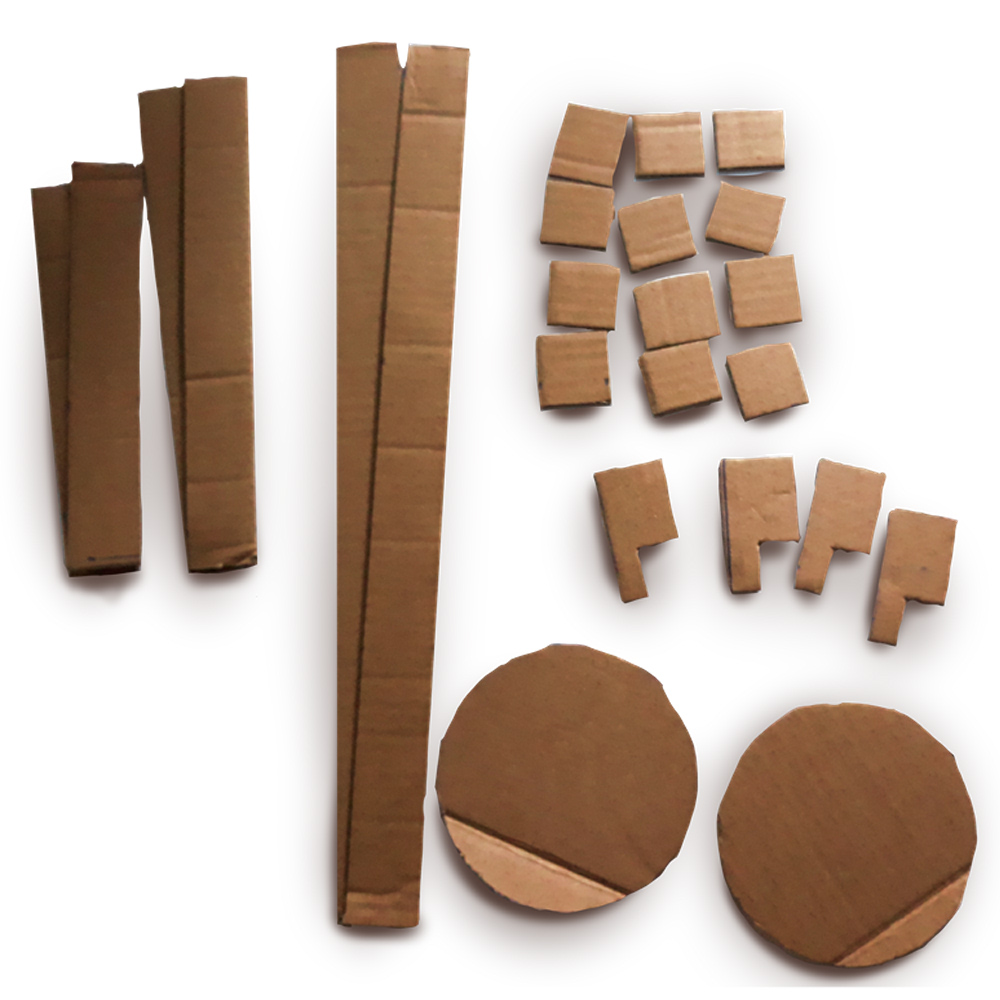
\includegraphics[width=5cm]{pappstucke.jpg}
\caption*{Stifte}
\end{figure}

}

\schritt{2}{Den Roboterarm bauen}{
Die Pappstreifen werden jetzt zusammengeklebt.
Dafür klebt ihr die jeweils beiden gleichlangen Streifen mit Heißkleber zusammen, sodass ihr nun zwei 30cm, ein 15cm und ein 12cm langes Pappstück habt.
Die vier Pappteile klebt ihr übereinander zu einem Klotz. An diesem können später die Stifte befestigt werden.\\

Jetzt wird es ein bisschen knifflig.
Die Pappteile müssen zu einem Arm zusammengebaut werden. Dabei bilden zwei kleine Pappquadrae und ein Zahnstocher ein Gelenk, das die Pappteile miteinander verbindet.
Am besten orientiert ihr euch an der folgenden Grafik:


Falls ihr nicht weiterwisst, gibt es auch eine ausführlichere Beschreibung auf https://tuduu.org/projekt/automatischer-malroboter .
Tipp: Den Pappblock klebt ihr auf die Unterseite des Arms, also nicht die Fläche, auf welcher der zweite Pappstreifen aufliegt.


Wenn alles zusammengesteckt und verbunden ist, testet euren Arm vorsichtig. Bewegt sich alles reibungslos?
Dann verklebt die Zahnstocher zum Schluss oben und unten mit einem Tropfen Heißkleber, dann hällt alles ein bisschen besser.
Die Pappkreise klebt ihr so auf die Reifen, dass die Pappstreifen ganz oben liegen.


%%%%%%%%%%%%%%%%%%%%%%%%%%%%%%





}


\subsection{Verbindung mit RaspberryPi}

\begin{center}
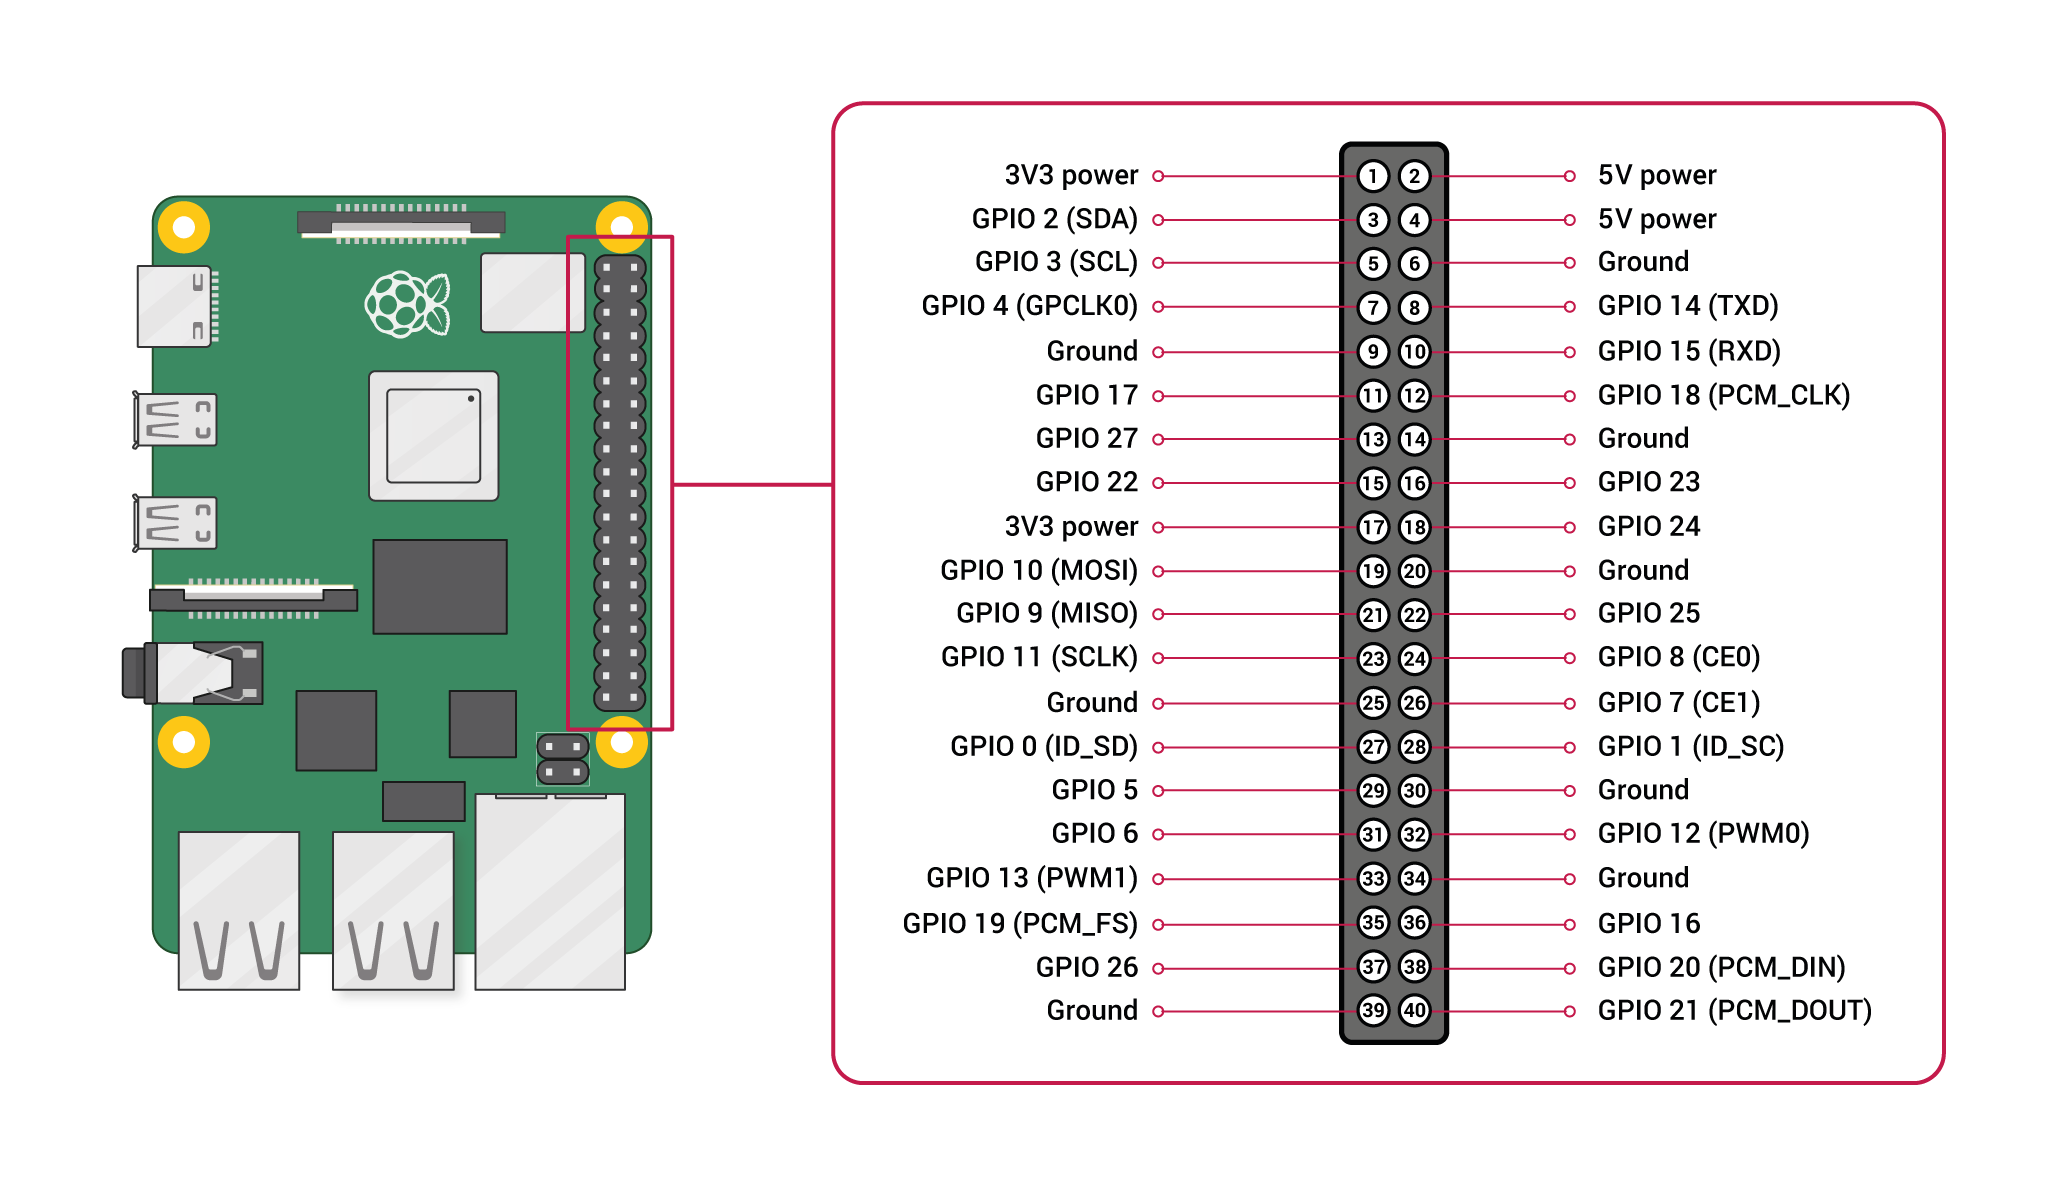
\includegraphics[width=\textwidth]{rpi_gpio_pinout.png}
\end{center}

\subsubsection{Verbindung Motor mit Treiber}
\subsubsection{Verbindung Treiber mit RaspberryPi}

\subsection{Programmierung}
\subsection{Programm A (Beispiel)}
\subsection{Programm B}
